\section{Calculs approchés d'intégrales}

Nous abordons dans cette section quelques méthodes dont le but est d’estimer la valeur numérique de l'intégrale d'une fonction donnée $f$ définie sur un domaine borné $\interff{a}{b}$:
\[
I = \int_a^b f(t) \d t.
\]
Ces méthodes nous fourniront une valeur approchée $\widetilde{I}$ de l'intégrale $I$ de sorte que \chevron{$\widetilde{I} \approx I$}. \\
Soient $a$ et $b$ deux réels tels que $a < b$. Pour tout entier naturel $p$ non nul, on note $(x_i)_{i\in\llbracket 0, p \rrbracket}$ la subdivision régulière de $[a, b]$ de pas $\frac{b-a}{p}$. Ainsi, pour tout $i \in \llbracket 0, p \rrbracket$,
\[
x_i = a + i\, \frac{b-a}{p}.
\]

\begin{defi}
Une méthode d'intégration est d'\emph{ordre} au moins $n$ si elle est exacte (\emph{i.e.} $\widetilde{I} = I$) pour les polynômes de degrés inférieurs ou égaux $n$ et non exacte pour au moins un polynôme de degré $n+1$.
\end{defi}

%-----------
\subsection{Méthode des rectangles à gauche}

La méthode des rectangles à gauche consiste, pour chacun des intervalles de la subdivision, à approcher l'aire sous la courbe représentative de $f$ par celle d'un rectangle dont la hauteur correspond à la valeur de $f$ sur la borne de gauche. Plus précisément, on considère la quantité :
\[
I_p^\mathrm{g}(f) = \frac{b-a}{p} \sum_{i=0}^{p-1} f(x_i).
\]

\begin{marginfigure}[-3cm]
    \centering
    %https://tex.stackexchange.com/questions/476702/riemann-sum-approaches-area-under-curve

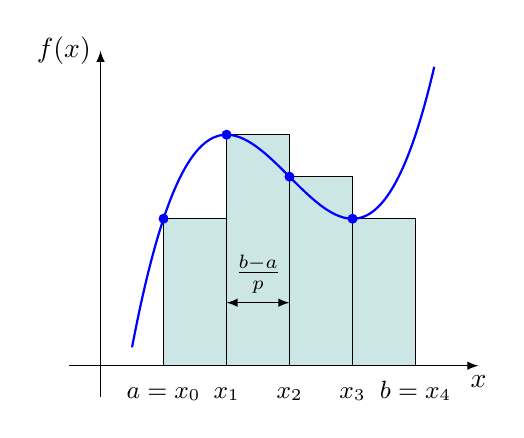
\begin{tikzpicture}[scale=0.8,declare function={f(\x)=((1/3)*(\x)^(3)-3*(\x)^(2)+8*\x-3;}]
\coordinate (start) at (.8,{f(.8)});
\coordinate (x0) at (1,{f(1)});
\coordinate (x1) at (2,{f(2)});
\coordinate (x2) at (3,{f(3)});
\coordinate (x3) at (4,{f(4)});
\coordinate (x4) at (5,{f(5)});
\coordinate (end) at (5.05,{f(5.05)});
\draw[fill=teal!20!white] (1,0) rectangle (2,{f(1)});
\draw[fill=teal!20!white] (2,0) rectangle (3,{f(2)});
\draw[fill=teal!20!white] (3,0) rectangle (4,{f(3)});
\draw[fill=teal!20!white] (4,0) rectangle (5,{f(4)});
%\draw (5,0)--(5,{f(5)});
\draw [-latex] (-0.5,0) -- (6,0) node (xaxis) [below] {$x$};
\draw [-latex] (0,-0.5) -- (0,5) node [left] {$f(x)$};
\foreach \x/\xtext in {1/a=x_0 ,2/x_1, 3/x_2 , 4/x_3 , 5/b=x_4}
 \draw[xshift=\x cm] node[below=2pt,fill=white,font=\small, anchor=south, yshift=-5mm] {$\xtext$};
\draw[domain=.5:5.3,samples=200,variable=\x,blue,thick] plot ({\x},{f(\x)});                 
\foreach \n in {0,1,2,3}
\draw[blue,fill=blue] (x\n) circle (2pt) node[font=\normalsize] {$ $};    
\draw[latex-latex] (2,1)--(3,1) node[midway, anchor=south] {$\frac{b-a}{p}$};      
\end{tikzpicture}
    \caption{Illustration de la méthode des rectangles à gauche}
\end{marginfigure}
\marginnote[3cm]{Animation de la méthode des rectangles à gauche : \url{https://acamanes.github.io/psi/psi_doc/animations/integration_segment/01-methode_des_rectangles_a_gauche.mp4}}

\begin{prop}
La méthode des rectangles à gauche est d'ordre $0$. De plus, si $f$ est de classe $\mathscr{C}^1$, l'erreur commise est en $O(1/p)$.
\end{prop}

\begin{exercice}
Soit $f$ une fonction de classe $\mathscr{C}^1$ sur le segment $\interff{a}{b}$. On note $F$ une primitive de $f$ et $M_1 = \sup_{\interff{a}{b}} \module{f'}$.
\begin{questions}
\item Montrer que
\[
\forall i \in \interent{0}{p-1},\quad 
\module{F(x_{i+1}) - F(x_i) - (x_{i+1} - x_i) F'(x_i)} \leqslant \frac{M_1}{2} (x_{i+1}-x_i)^2.
\]

\item En déduire que
\[
\module{\int_{\interff{a}{b}} f(t) \d t - I_p^\mathrm{g}(f)}
\leqslant \frac{M_1 (b-a)^2}{2 p}.
\]

\item Utiliser la méthode des rectangles à gauche pour calculer une valeur approchée de l'intégrale de la fonction $x \mapsto x - a$.

\item Conclure.
\end{questions}
\end{exercice}

\begin{elemsolution}

\begin{reponses}
\item Il s'agit d'une application de la formule de \textsc{Taylor} avec reste intégal.

\item En utilisant la relation de \textsc{Chasles},
\begin{align*}
\module{\int_{\interff{a}{b}} f(t) \d t - I_p^\mathrm{g}(f)}
&\leqslant \sum_{i=1}^{p-1} \module{\int_{\interff{x_i}{x_{i+1}}} f(x) \d x - (x_{i+1} - x_i) f(x_i)}\\
&\leqslant \sum_{i=1}^{p-1} \frac{M_1}{2} (x_{i+1} - x_i)^2
% &\leq \frac{M_1}{2} (b - a) \sum_{i=1}^{p-1} (x_{i+1} - x_i)\\
\leqslant \frac{M_1 (b-a)^2}{2 p}.
\end{align*}

\item On remarque que, dans ce cas, $M_1 = b - a$ et la borne est atteinte.

\item La méthode des rectangles à gauche est exacte si $f$ est constante. Cependant, le calcul précédent montre que si $\fonctionligne[f]{x}{x - a}$, alors la méthode ne donne pas la valeur exacte de l'intégrale. La méthode est donc d'ordre $0$.
\end{reponses}
\end{elemsolution}

%-----------
\subsection{Méthode des rectangles médians}

La méthode des rectangles médians consiste, pour chacun des intervalles de la subdivision, à approcher l'aire sous la courbe représentative de $f$ par celle d'un rectangle dont la hauteur correspond à la valeur de $f$ au milieu de la subdivision. Plus précisément, on considère la quantité :
\[
I_p^\mathrm{m}(f) = \frac{b-a}{p} \sum_{i=0}^{p-1} f\left(\frac{x_i + x_{i+1}}{2} \right).
\]

\begin{prop}
La méthode des rectangles médians est d'ordre $1$. De plus, si $f$ est de classe $\mathscr{C}^2$, l'erreur commise est en $O(1/p^2)$.
\end{prop}

\begin{marginfigure}[-3cm]
    \centering
    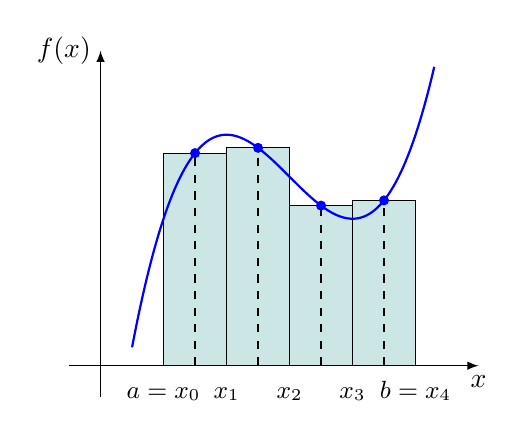
\begin{tikzpicture}[scale=0.8,declare function={f(\x)=((1/3)*(\x)^(3)-3*(\x)^(2)+8*\x-3;}]
\coordinate (start) at (.8,{f(.8)});
\coordinate (x0) at (1.5,{f(1.5)});
\coordinate (x1) at (2.5,{f(2.5)});
\coordinate (x2) at (3.5,{f(3.5)});
\coordinate (x3) at (4.5,{f(4.5)});
\coordinate (x4) at (5.5,{f(5.5)});
\coordinate (end) at (5.05,{f(5.05)});
\draw[fill=teal!20!white] (1,0) rectangle (2,{f(1.5)});
\draw[fill=teal!20!white] (2,0) rectangle (3,{f(2.5)});
\draw[fill=teal!20!white] (3,0) rectangle (4,{f(3.5)});
\draw[fill=teal!20!white] (4,0) rectangle (5,{f(4.5)});

\draw[dashed] (1.5, 0) -- (1.5,{f(1.5)});
\draw[dashed] (2.5, 0) -- (2.5,{f(2.5)});
\draw[dashed] (3.5, 0) -- (3.5,{f(3.5)});
\draw[dashed] (4.5, 0) -- (4.5,{f(4.5)});

\draw [-latex] (-0.5,0) -- (6,0) node (xaxis) [below] {$x$};
\draw [-latex] (0,-0.5) -- (0,5) node [left] {$f(x)$};
\foreach \x/\xtext in {1/a=x_0 ,2/x_1, 3/x_2 , 4/x_3 , 5/b=x_4}
 \draw[xshift=\x cm] node[below=2pt,fill=white,font=\small, anchor=south, yshift=-5mm] {$\xtext$};
\draw[domain=.5:5.3,samples=200,variable=\x,blue,thick] plot ({\x},{f(\x)});                 
\foreach \n in {0,1,2,3}
\draw[blue,fill=blue] (x\n) circle (2pt) node[font=\normalsize] {$ $};    
% \draw[latex-latex] (2,1)--(3,1) node[midway, anchor=south] {$\frac{b-a}{p}$};      
\end{tikzpicture}
    \caption{Illustration de la méthode des rectangles médians}
\end{marginfigure}
\marginnote[3cm]{Animation de la méthode des rectangles médians : \url{https://acamanes.github.io/psi/psi_doc/animations/integration_segment/02-methode_des_rectangles_medians.mp4}}

\begin{exercice}
Soit $f$ une fonction de classe $\mathscr{C}^2$ sur le segment $\interff{a}{b}$. On note $F$ une primitive de $f$ et $M_2 = \sup_{\interff{a}{b}} \module{f''}$. Pour tout entier $i \in \interent{0}{p-1}$, on pose $\gamma_i = \frac{x_i + x_{i+1}}{2}$ le milieu du segment $\interff{x_i}{x_{i+1}}$.
\begin{questions}
\item Montrer que
\[
\forall i \in \interent{0}{p-1},\quad 
(x_{i+1} - x_i) f(\gamma_i) = \int_{x_i}^{x_{i+1}} \left(f(\gamma_i) + (t - \gamma_i) f'(\gamma_i) \right) \d t.
\]    

\item Montrer que
\[
\forall i \in \interent{0}{p-1},\quad 
\module{F(x_{i+1}) - F(x_i) - (x_{i+1} - x_i) F'(\gamma_i)} \leqslant \frac{M_2}{24} (x_{i+1} - x_i)^3.
\]

\item En déduire que
\[
\module{\int_{[a,b]} f(t) \d t- I_p^\mathrm{m}(f)} \leqslant \frac{M_2 (b-a)^3}{24 p^2}.
\]

\item Appliquer l'inégalité précédente à la fonction $x \mapsto (x - a)^2$.

\item Conclure.
\end{questions}
\end{exercice}


\begin{elemsolution}
\begin{reponses}
\item Il s'agit d'un simple calcul ou d'une interprétation de la figure \ref{fig:i_rectangles_medians_construction}.

\item Ainsi, d'après la formule de \textsc{Taylor} avec reste intégral,
\begin{align*}
\module{F(x_{i+1}) - F(x_i) - (x_{i+1} - x_i) F'(\gamma_i)}
&= \module{\int_{x_i}^{x_{i+1}} \left(f(t) - f(\gamma_i) - (t - \gamma_i) f'(\gamma_i)\right) \d t} \\
&\leqslant \frac{M_2}{24} (x_{i+1} - x_i)^3.
\end{align*}

\begin{marginfigure}[0cm]
    \centering
    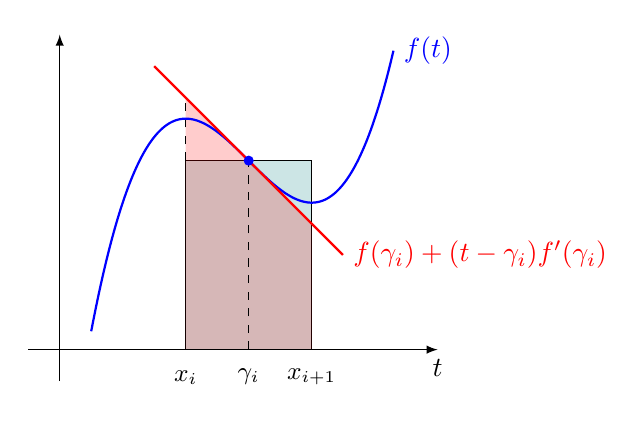
\begin{tikzpicture}[scale=0.8,declare function={f(\x)=((1/3)*(\x)^(3)-3*(\x)^(2)+8*\x-3;}, declare function={g(\x)=-\x+6;},]
\coordinate (xm) at (3,{f(3)});

\draw[fill=teal!20!white] (2,0) rectangle (4,{f(3)});
\fill[red, opacity=0.2,ultra thick] (2,0) -- (2,{g(2)}) -- (4, {g(4)}) -- (4, 0);

\draw[dashed] (3, 0) -- (3,{f(3)});
\draw[dashed] (2, {f(3)}) -- (2,{g(2)});

\draw [-latex] (-0.5,0) -- (6,0) node (xaxis) [below] {$t$};
\draw [-latex] (0,-0.5) -- (0,5);
% \foreach \x/\xtext in {1/a=x_0 ,2/x_1, 3/x_2 , 4/x_3 , 5/b=x_4}
\draw[xshift=2 cm] node[below=2pt,fill=white,font=\small, anchor=south, yshift=-5mm] {$x_i$};
\draw[xshift=3 cm] node[below=2pt,fill=white,font=\small, anchor=south, yshift=-5mm] {$\gamma_i$};
\draw[xshift=4 cm] node[below=2pt,fill=white,font=\small, anchor=south, yshift=-5mm] {$x_{i+1}$};
\draw[domain=.5:5.3,samples=200,variable=\x,blue,thick] plot ({\x},{f(\x)}) node[right] {$f(t)$};  
\draw[domain=1.5:4.5,samples=200,variable=\x,red,thick] plot ({\x},{g(\x)}) node[right] {$f(\gamma_i) + (t - \gamma_i) f'(\gamma_i)$}; 
% \foreach \n in {0,1,2,3}
\draw[blue,fill=blue] (xm) circle (2pt) node[font=\normalsize] {$ $};    
% \draw[latex-latex] (2,1)--(3,1) node[midway, anchor=south] {$\frac{b-a}{p}$};      
\end{tikzpicture}
    \caption{}
    \label{fig:i_rectangles_medians_construction}
\end{marginfigure}

\item Comme pour la méthode des rectangles à gauche, il s'agit d'une application de la formule de \textsc{Chasles}.

\item On montre que la borne est atteinte pour $f : x \mapsto (x - a)^2$.

\item La méthode des rectangles médians est exacte si $f$ est un polynôme de degré $1$. Cependant, si $f$ est la fonction $x \mapsto (x - a)^2$, le calcul précédent montre que la méthode des rectangles médians ne donne pas la valeur exacte de l'intégrale. La méthode est donc d'ordre $1$.
\end{reponses}
\end{elemsolution}

%-----------
\subsection{Méthode des trapèzes}

La méthode des trapèzes consiste, pour chacun des intervalles de la subdivision, à approcher l'aire sous la courbe représentative de $f$ par celle d'un trapèze. Plus précisément, on considère la quantité :
\[
I_p^\mathrm{t}(f) =  \frac{b-a}{p} \sum_{i=0}^{p-1} \frac{f(x_i) + f(x_{i+1})}{2}.
\]

\begin{marginfigure}[0cm]
    \centering
    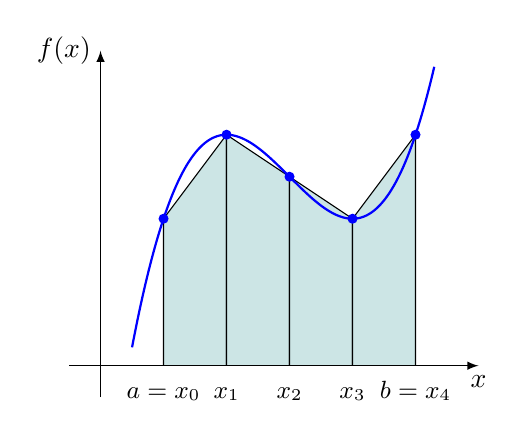
\begin{tikzpicture}[scale=0.8,declare function={f(\x)=((1/3)*(\x)^(3)-3*(\x)^(2)+8*\x-3;}]
\coordinate (start) at (.8,{f(.8)});
\coordinate (x0) at (1,{f(1)});
\coordinate (x1) at (2,{f(2)});
\coordinate (x2) at (3,{f(3)});
\coordinate (x3) at (4,{f(4)});
\coordinate (x4) at (5,{f(5)});
\coordinate (end) at (5.05,{f(5.05)});

\draw[fill=teal!20!white] (1,0)--(1,{f(1)})--(2,{f(2)})--(2,0);
\draw[fill=teal!20!white] (2,0)--(2,{f(2)})--(3,{f(3)})--(3,0);
\draw[fill=teal!20!white] (3,0)--(3,{f(3)})--(4,{f(4)})--(4,0);
\draw[fill=teal!20!white] (4,0)--(4,{f(4)})--(5,{f(5)})--(5,0);


%\draw (5,0)--(5,{f(5)});
\draw [-latex] (-0.5,0) -- (6,0) node (xaxis) [below] {$x$};
\draw [-latex] (0,-0.5) -- (0,5) node [left] {$f(x)$};
\foreach \x/\xtext in {1/a=x_0 ,2/x_1, 3/x_2 , 4/x_3 , 5/b=x_4}
 \draw[xshift=\x cm] node[below=2pt,fill=white,font=\small, anchor=south, yshift=-5mm] {$\xtext$};
\draw[domain=.5:5.3,samples=200,variable=\x,blue,thick] plot ({\x},{f(\x)});                 
\foreach \n in {0,1,2,3,4}
\draw[blue,fill=blue] (x\n) circle (2pt) node[font=\normalsize] {$ $};    
% \draw[latex-latex] (2,1)--(3,1) node[midway, anchor=south] {$\frac{b-a}{p}$};      
\end{tikzpicture}
    \caption{Illustration de la méthode des trapèzes}
\end{marginfigure}
\marginnote[6cm]{Animation de la méthode des trapèzes : \url{https://acamanes.github.io/psi/psi_doc/animations/integration_segment/03-methode_des_trapezes.mp4}}

\begin{prop}
La méthode des trapèzes est d'ordre $1$. De plus, si $f$ est de classe $\mathscr{C}^2$, l'erreur commise est en $O(1/p^2)$.
\end{prop}

\begin{exercice}
Soit $f$ une fonction de classe $\mathscr{C}^2$. On note $M_2 = \sup_{[a,b]} \module{f''}$. Pour tout $i \in \interent{0}{p-1}$, on note $\phi_i$ l'approximation affine sur $\interff{x_i}{x_{i+1}}$ de $f$ et $g_i = f - \phi_i$.
\begin{questions}
\item Montrer que
\[
\forall i \in \interent{0}{p-1},\quad 
\int_{x_i}^{x_{i+1}} f''(t)\,(t - x_i) (x_{i+1} - t) \d t = - 2 \int_{x_i}^{x_{i+1}} g_i(t) \d t.
\]

\item Montrer que
\[
\forall i \in \interent{0}{p-1},\quad 
\module{\int_{x_i}^{x_{i+1}} f(t) \d t - I_p^\mathrm{t}(f)}
\leqslant \frac{M_2}{2} \cdot \frac{(b - a)^3}{6}.
\]

\item En déduire que
\[
\module{\int_{[a,b]} f(t) \d t - I_p^\mathrm{t}(f)} \leqslant \frac{M_2 (b-a)^3}{12 p^2}.
\]

\item Appliquer l'égalité précédente à la fonction $x \mapsto (x - a)^2$.

\item Conclure.
\end{questions}
\end{exercice}

\begin{elemsolution}
\begin{reponses}
\item Il suffit d'effectuer deux intégrations par parties successives.

\item D'après la relation précédente, on établit que
\begin{align*}
\module{\int_{x_i}^{x_{i+1}} f(t) \d t - I_p^\mathrm{t}(f)}
&\leqslant \int_{x_i}^{x_{i+1}} \module{f(t) - \phi_i(t)} \d t\\
&\leqslant \frac{M_2}{2} \int_{x_i}^{x_{i+1}} (t - x_i) (x_{i+1} - t) \d t
\leqslant \frac{M_2}{2} \cdot \frac{(b - a)^3}{6}.
\end{align*}

\item Comme pour les méthodes précédentes, on utilise la relation de \textsc{Chasles}.

\item On montre que cette borne est atteinte pour $f : x \mapsto (x - a)^2$.

\item La méthode des trapèzes est exacte si $f$ est un polynôme de degré $1$. Cependant, si $f$ est la fonction $x \mapsto (x - a)^2$, le calcul précédent montre qur la méthode des trapèzes ne donne pas la valeur exacte de l'intégrale. La méthode est donc d'ordre $2$.
\end{reponses}
\end{elemsolution}

\begin{marginfigure}[-1cm]
\begin{subfigure}{.5\textwidth}
    \centering
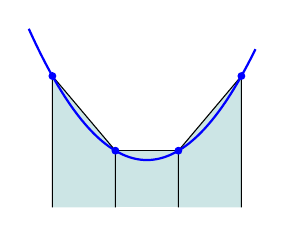
\begin{tikzpicture}[scale=0.6]

\pgfmathdeclarefunction{f}{1}{%
    \pgfmathparse{((#1 - 3) / 1.5)^2 + 1}%
}
% ,declare function={f(\x)=((\x-3)/1.5)^2+1;}]
\coordinate (start) at (.8,{f(.8)});
\coordinate (x0) at (1,{f(1)});
\coordinate (x1) at (1+4/3,{f(1+4/3)});
\coordinate (x2) at (1+8/3,{f(1+8/3)});
\coordinate (x3) at (1+12/3,{f(1+12/3)});
\coordinate (end) at (5.05,{f(5.05)});

\draw[fill=teal!20!white] (1,0)--(1,{f(1)})--(1+4/3,{f(1+4/3)})--(1+4/3,0);
\draw[fill=teal!20!white] (1+4/3,0)--(1+4/3,{f(1+4/3)})--(1+8/3,{f(1+8/3)})--(1+8/3,0);
\draw[fill=teal!20!white] (1+8/3,0)--(1+8/3,{f(1+8/3)})--(5,{f(5)})--(5,0);

\draw[domain=.5:5.3,samples=200,variable=\x,blue,thick] plot ({\x},{f(\x)});                 

\draw[blue,fill=blue] (x0) circle (2pt);    
\draw[blue,fill=blue] (x1) circle (2pt);    
\draw[blue,fill=blue] (x2) circle (2pt);    
\draw[blue,fill=blue] (x3) circle (2pt);    

\end{tikzpicture}
    \caption{Cas convexe}
\end{subfigure}%
\begin{subfigure}{.5\textwidth}
    \centering
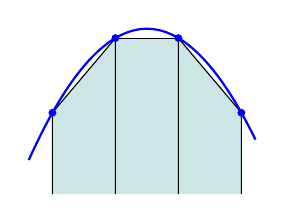
\begin{tikzpicture}[scale=0.6
% ,declare function={f(\x)=-((\x-3)/1.5)^2+3.5;}
]

\pgfmathdeclarefunction{f}{1}{%
    \pgfmathparse{-((#1 - 3) / 1.5)^2 + 3.5}%
}
\coordinate (start) at (.8,{f(.8)});
\coordinate (x0) at (1,{f(1)});
\coordinate (x1) at (1+4/3,{f(1+4/3)});
\coordinate (x2) at (1+8/3,{f(1+8/3)});
\coordinate (x3) at (1+12/3,{f(1+12/3)});
\coordinate (end) at (5.05,{f(5.05)});

\draw[fill=teal!20!white] (1,0)--(1,{f(1)})--(1+4/3,{f(1+4/3)})--(1+4/3,0);
\draw[fill=teal!20!white] (1+4/3,0)--(1+4/3,{f(1+4/3)})--(1+8/3,{f(1+8/3)})--(1+8/3,0);
\draw[fill=teal!20!white] (1+8/3,0)--(1+8/3,{f(1+8/3)})--(5,{f(5)})--(5,0);

\draw[domain=.5:5.3,samples=200,variable=\x,blue,thick] plot ({\x},{f(\x)});                 

\draw[blue,fill=blue] (x0) circle (2pt);    
\draw[blue,fill=blue] (x1) circle (2pt);    
\draw[blue,fill=blue] (x2) circle (2pt);    
\draw[blue,fill=blue] (x3) circle (2pt);  

\end{tikzpicture}
    \caption{Cas concave}
\end{subfigure}
\caption{Illustration de la remarque \ref{remarquemethodetrapezes}}
\end{marginfigure}

\begin{remarque}\label{remarquemethodetrapezes}
Lorsque $f$ est de classe $\mathscr{C}^2$ et convexe (resp. concave), alors $f'' \geqslant 0$ (resp. $\leqslant 0$) et, pour tout $p$ entier naturel, \mbox{$\int_{[a,b]} f \leqslant I_p^\mathrm{t}(f)$} (resp. \mbox{$\int_{[a,b]} f \geqslant I_p^\mathrm{t}(f)$}). On obtient ainsi une valeur approchée par excès (resp. par défaut) de l'intégrale.
\end{remarque}

\subsection{Méthode de \textsc{Simpson}}

La méthode de \textsc{Simpson} consiste, pour chacun des intervalles de la subdivision, à approcher la fonction $f$ par un polynôme de degré inférieur ou égal à $2$. Plus précisément, on considère la quantité :
\[
I_p^\mathrm{s}(f) = \frac{b-a}{6 p} \sum_{i=0}^{p-1} \left[f(x_i)+ 4 f\left(\frac{x_i + x_{i+1}}{2}\right) + f(x_{i+1})\right].
\]

\begin{prop}
Dans la méthode de \textsc{Simpson}, si $f$ est de classe $\mathscr{C}^4$, l'erreur commise est en $O(1/p^4)$.
\end{prop}

\todoinline{Tu aurais le courage de vérifier le calcul suivant ?}

\begin{exercice}
Soit $f$ une fonction de classe $\mathscr{C}^4$ sur le segment $\interff{a}{b}$. On note $F$ une primitive de $f$ et $M_4 = \sup_{[a,b]} \big\vert f^{(4)} \big\vert$.

Pour tout $i \in \interent{0}{p-1}$, notons $\gamma_i = \frac{x_i + x_{i+1}}{2}$ le milieu de la subdivision et $h_i = \frac{x_{i+1} - x_i}{2}$ la moitié de sa longueur.
\begin{questions}
\item Montrer que pour tout $i \in \interent{0}{p-1}$,
\[
F(x_{i+1}) - F(x_i)
= \begin{multlined}[t] 
2 h_i f(\gamma_i) + \frac{h_i{}^3}{3} f''(\gamma_i) \\
+ \frac{h_i{}^5}{24} \int_0^1 (1 - t)^4 \mathopen{}\left[f^{(4)}(\gamma_i + t h_i) + f^{(4)}(\gamma_i - t h_i)\right] \d t.
\end{multlined} 
\]

\item Montrer que pour tout $i \in \interent{0}{p-1}$,
\[
\module{f(x_{i+1}) + f(x_i) - 2 f(\gamma_i) - h_i{}^2 f(\gamma_i)} \leqslant \frac{h_i{}^4 \times 2 M_4}{4!}.
\]

\item En déduire que pour tout $i \in \interent{0}{p-1}$,
\[
\module{\int_{x_i}^{x_{i+1}} f(t) \d t - \frac{h_i}{3} \left[f(x_i) + 4 f(\gamma_i) + f(x_{i+1})\right]}
\leqslant \frac{(x_{i+1} - x_i)^5}{720}.
\]

\item Conclure.
\end{questions}
\end{exercice}

\begin{elemsolution}
\begin{reponses}
\item D'après la formule de \textsc{Taylor} avec reste intégral appliquée à une primitive $F$ de $f$ et en remarquant que $x_{i+1} = \gamma_i + h_i$ et $x_i = \gamma_i - h_i$,
\begin{align*}
F(x_{i+1}) = F(\gamma_i + h_i)
&= \begin{aligned}[t]F(\gamma_i) + h_i f(\gamma_i) + \frac{h_i{}^2}{2} f'(\gamma_i) + \frac{h_i{}^3}{6} f''(\gamma_i) + \frac{h_i{}^4}{24} f'''(\gamma_i) \\ + \frac{h_i{}^5}{24} \int_0^1 (1 - t)^4 f^{(4)}(\gamma_i + t h_i) \d t,\\
\end{aligned} \\
\intertext{et}
F(x_i) = F(\gamma_i - h_i)
&= \begin{aligned}[t]F(\gamma_i) - h_i f(\gamma_i) + \frac{h_i{}^2}{2} f'(\gamma_i) - \frac{h_i{}^3}{6} f''(\gamma_i) + \frac{h_i{}^4}{24} f'''(\gamma_i) \\ - \frac{h_i{}^5}{24} \int_0^1 (1 - t)^4 f^{(4)}(\gamma_i - t h_i) \d t.
\end{aligned}
\end{align*}
Le résultat s'obtient en soustrayant les deux relations précédentes.


\item On applique la formule de \textsc{Taylor} avec reste intégral à la fonction $f$ sur $[\gamma_i - h_i, \gamma_i]$ et $[\gamma_i, \gamma_i + h_i]$.

\item Finalement,
\begin{align*}
\module{\int_{x_i}^{x_{i+1}} f(t) \d t - \frac{h_i}{3} \left[f(x_i) + 4 f(\gamma_i) + f(x_{i+1})\right]}
&\leqslant \module{\frac{h_i}{3} \left[f(x_i) - 2 f(\gamma_i) + f(x_{i+1}) - h_i{}^2 f''(\gamma_i)\right]} + \frac{h_i{}^5 2 M_4}{5! p^5}\\
&\leqslant h_i{}^5 \left[\frac{2}{3 \times 4!} + \frac{2}{5!}\right]\\
&\leqslant \frac{2 h_i{}^5}{45}
\leqslant \frac{(x_{i+1} - x_i)^5}{720}.
\end{align*}

\item On conclut à l'aide de la relation de \textsc{Chasles} :
\[
\module{\int_a^b f(t) \d t - I_p^\mathrm{s}(f)} \leq \frac{M_4 (b-a)^5}{720 p^4}.
\]
% \[
% \module{I_p^s(f) - \int_a^b f(t) \d t} \leq \frac{M_4 (b-a)^5}{2880 p^4}.
% \]
\end{reponses}
\end{elemsolution}

\begin{figure}[H]
    \centering
    \newcommand*{\parabolaShading}[6]{
\fill [cyan!10, domain=(#1:#5), variable=\x] (#1,0)  -- plot 
    (  {\x},{(#2*(\x-#3)*(\x-#5)/((#1-#3)*(#1-#5)))+
            (#4*(\x-#1)*(\x-#5)/((#3-#1)*(#3-#5)))+
            (#6*(\x-#1)*(\x-#3)/((#5-#1)*(#5-#3)))} )
    -- (#5,0) -- cycle;
}
\newcommand*{\parabolaLines}[6]{
\draw plot [domain=(#1-0.25):(#5+0.25)] %can be adjusted
    (   {\x},{(#2*(\x-#3)*(\x-#5)/((#1-#3)*(#1-#5)))+
            (#4*(\x-#1)*(\x-#5)/((#3-#1)*(#3-#5)))+
            (#6*(\x-#1)*(\x-#3)/((#5-#1)*(#5-#3)))} );
}
\newcommand*{\shadeWithBoundedDomainAndColor}[9]{ %first 6 are points; 7,8 are domain; 9 is color
\fill [#9, domain=(#7:#8), variable=\x] (#7,0)  -- plot 
    (  {\x},{(#2*(\x-#3)*(\x-#5)/((#1-#3)*(#1-#5)))+
            (#4*(\x-#1)*(\x-#5)/((#3-#1)*(#3-#5)))+
            (#6*(\x-#1)*(\x-#3)/((#5-#1)*(#5-#3)))} )
    -- (#8,0) -- cycle;
}

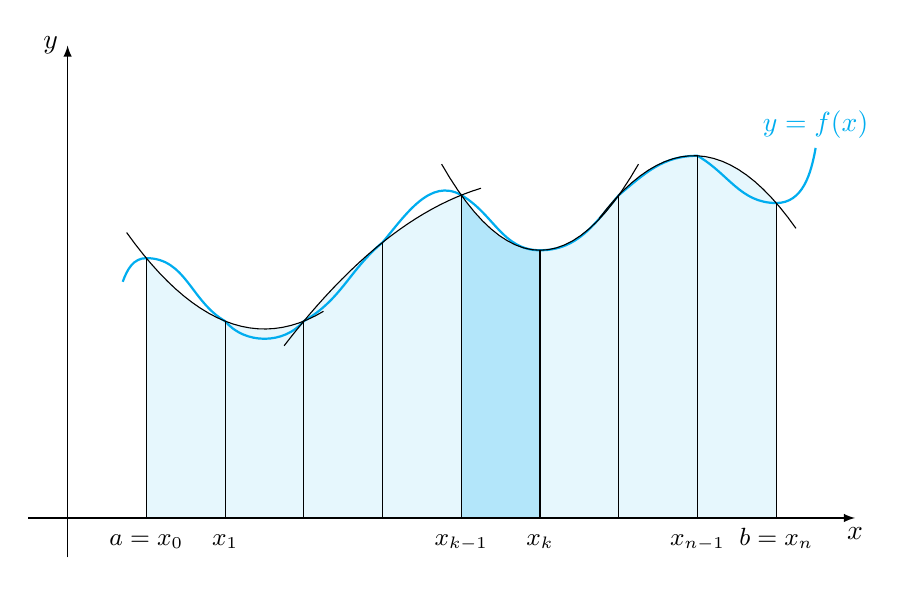
\begin{tikzpicture}
\coordinate (p1) at (0.7,3);
\coordinate (p2) at (1,3.3);
\coordinate (p3) at (2,2.5);
\coordinate (p4) at (3,2.5);
\coordinate (p5) at (4,3.5);
\coordinate (p6) at (5,4.1);
\coordinate (p7) at (6,3.4);
\coordinate (p8) at (7,4.1);
\coordinate (p9) at (8,4.6);
\coordinate (p10) at (9,4);
\coordinate (p11) at (9.5,4.7);

%Shading
\parabolaShading{1}{3.3}{2}{2.5}{3}{2.5}
%\parabolaShading{2}{2.5}{3}{2.5}{4}{3.5}
\parabolaShading{3}{2.5}{4}{3.5}{5}{4.1}
%\parabolaShading{4}{3.5}{5}{4.1}{6}{3.4}
\parabolaShading{5}{4.1}{6}{3.4}{7}{4.1}
%\parabolaShading{6}{3.4}{7}{4.1}{8}{4.6}
\parabolaShading{7}{4.1}{8}{4.6}{9}{4}
\shadeWithBoundedDomainAndColor{5}{4.1}{6}{3.4}{7}{4.1}{5}{6}{cyan!30}

% the curve
\draw[thick,cyan]
  (p1) to[out=70,in=180] (p2) to[out=0,in=150]
  (p3) to[out=-50,in=230] (p4) to[out=30,in=220]
  (p5) to[out=50,in=150] (p6) to[out=-30,in=180]
  (p7) to[out=0,in=230] (p8) to[out=40,in=180]
  (p9) to[out=-30,in=180] (p10) to[out=0,in=260] (p11);

%uncomment the rest for all of the parabolas
\parabolaLines{1}{3.3}{2}{2.5}{3}{2.5}
%\parabolaLines{2}{2.5}{3}{2.5}{4}{3.5}
\parabolaLines{3}{2.5}{4}{3.5}{5}{4.1}
%\parabolaLines{4}{3.5}{5}{4.1}{6}{3.4}
\parabolaLines{5}{4.1}{6}{3.4}{7}{4.1}
%\parabolaLines{6}{3.4}{7}{4.1}{8}{4.6}
\parabolaLines{7}{4.1}{8}{4.6}{9}{4}

% vertical lines and labels
\foreach \n/\texto in {2/{a=x_0},3/{x_1},4/{},5/{},6/{x_{k-1}},7/{x_k},8/{},9/{x_{n-1}},10/{b=x_n}}
{
  \draw (p\n|-0,0) -- (p\n);
  \node[below,text height=1.5ex,text depth=1ex,font=\small] at (p\n|-0,0) {$\texto$};
}
% The axes
\draw[-latex] (-0.5,0) -- (10,0) coordinate (x axis);
\draw[-latex] (0,-0.5) -- (0,6) coordinate (y axis);
% labels for the axes
\node[below] at (x axis) {$x$};
\node[left] at (y axis) {$y$};
% label for the function
\node[above,text=cyan] at (p11) {$y=f(x)$};

\end{tikzpicture}
    \caption{Illustration de la méthode de \textsc{Simpson}}
\end{figure}
\todoarmand{Figure à reprendre, pour l'instant reprise de \url{https://tex.stackexchange.com/questions/429634/parabola-through-three-points-with-tikz}}

\todoinline{Très bonne idée}

%-----------
\subsection{Et ensuite ?}

Nous constatons que pour chacune des méthodes précédentes la stratégie est identique :
\begin{itemize}
\item découper le segment en une subdivision régulière $a = x_0 \leqslant \cdots \leqslant x_n = b$,

\item sur chacun des intervalles de cette subdivision, approcher la fonction par une fonction dont l'intégrale est plus simple.

Sur l'intervalle $[x_i, x_{i+1}]$ : pour la méthode des rectangles, on approche la fonction par une droite horizontale, pour celle des trapèzes, par une droite affine passant par les points $(x_i, f(x_i))$ et $(x_{i+1}, f(x_{i+1}))$.
\end{itemize}

Plus généralement, on peut découper le segment $\interff{x_i}{x_{i+1}}$ en une subdivision régulière $x_i = y_{i,0} \leqslant \ldots \leqslant y_{i,p} \leqslant x_{i+1}$. On peut ensuite approcher la fonction par le polynôme d'interpolation de \textsc{Lagrange} qui passe par les points de coordonnées $(y_{i,0}, f(y_{i,0})), \ldots, (y_{i,p}, f(y_{i,p}))$.

Cette méthode est appelée \emph{méthode de \textsc{Newton}--\textsc{Cotes}}.

Plus précisément, on considère une subdivision $0 = y_0 \leqslant \cdots \leqslant y_p = 1$ de l'intervalle $\interff{0}{1}$ et on note $(L_0,\ldots,L_p)$ la famille des \hyperref[sec:polynomes_de_lagrange]{polynômes d'interpolation de \textsc{Lagrange}} associée à cette subdivision, i.e.
\[
\forall i \in \interent{0}{p},\quad L_i(X) = \prod_{j \neq i} \frac{X - y_j}{y_i - y_j}.
\]

On pose alors $\gamma_j = \int_0^1 L_j(t) \d t$.

On approche alors l'intégrale de $f$ sur $[x_i, x_{i+1}]$ par la somme
\[
I_p^i(f) = (x_{i+1} - x_i) \sum_{j=0}^p \gamma_j g(x_i + (x_{i+1} - x_i) y_j),
\]
puis l'intégrale sur le segment $\interff{a}{b}$ par
\[
I_p(f) = \sum_{i=0}^{n-1} (x_{i+1} - x_i) \bigg[ \sum_{j=0}^p \gamma_j f(x_i + (x_{i+1} - x_i) y_j) \bigg].
\] 

On peut montrer que :
\begin{itemize}
\item lorsque $n = 1$, on retrouve la formule des trapèzes.

\item lorque $n = 2$, on retrouve la méthode de \textsc{Simpson}.
\end{itemize}

On peut montrer que la méthode de \textsc{Simpson} est d'ordre $3$. On peut augmenter le nombre des n\oe{}uds où est évaluée la fonction à intégrer ($2$ n\oe{}uds pour la méthode des trapèzes, $3$ pour la méthode de \textsc{Simpson},\ldots). Cependant, lorsque le nombre de n\oe{}uds dépasse $8$, des coefficients négatifs apparaissent ce qui engendre des erreurs d'arrondis. \\

\begin{table}[]
    \centering
    \begin{tblr}{
    hlines,vlines,
    hline{2} = {2pt},
    cells={c}
    }
    \textbf{Méthode} & \textbf{Ordre} & \textbf{Vitesse de conv.} & \textbf{\textsc{Newton}--\textsc{Cotes}} \\
    À gauche & $0$ & $O(1/p)$ & X\\
    À droite & $0$ & $O(1/p)$ & X\\
    Médians & $1$ & $O(1/p^2)$ & X\\
    Trapèzes & $1$ & $O(1/p^2)$ & 1\\
    \textsc{Simpson} & $3$ & $O(1/p^4)$ & 2
    \end{tblr}
    \caption{Résumé des propriétés des méthodes de calculs approchés d’intégrales}
\end{table} % margintable

\todoinline{
Je veux bien que tu t'occupes de ces deux points rapides, je ne maîtrise pas encore les différentes fonctions.

Mettre ici un lien vers un thème sur les polynômes d'interpolation de Lagrange.

On pourrait ajouter vers le livre Demailly - Analyse numérique et équations différentielles}
